\chapter{Introduction and Research Questions}
\section{Introduction}
Inactive and sedentary lifestyles are becoming a big issue around the world. “People are spending more and more time doing sedentary activities. During our leisure time, we are often sitting: while using a computer or other device, watching TV, or playing video games.”\cite{NIH}. Most of the jobs are becoming increasingly sedentary as well, as most jobs consists of long days in front of a desk. The situation is similar for the younger generation as they spend long days sitting at schools or universities. 

Sitting promotes deconditioning, which negatively affects employees’ abilities to meet the demands of increasingly physical workloads.\cite{Lurati} The average person spends a big portion of their day sitting still and prolonged sitting and sedentary lifestyles may lead to premature aging and contribute to chronic disease, prelude to lost productivity.(ibid). Not only are people sedentary, they are also inactive during their off time. An inactive lifestyle is a lifestyle with a lot of sitting and lying down with very little to no exercise \cite{NIH2} .

The world health organization (WHO) lists insufficient activity as one of the leading risk factors for death worldwide.  Insufficient activity is a key risk factor for many diseases like cardiovascular diseases, cancer and diabetes. \cite{WHO}. They state that more than 80\% of the world’s adolescent population is not active enough, and more than 25\% of the adult population. The world health organization recommends that adults should do at least 150 minutes of moderate-intensity physical activity a week.  Physical activities like running, cycling or playing sports can decrease the health and disease risks associated with a sedentary lifestyle. 

Another way of encouraging physical activity is to organize exercise, a physical activity that is planned, structured, and repetitive and has as a final or intermediate objective the improvement or maintenance of physical fitness \cite{Garber2011}. Exercise increases the physical fitness, which is the ability to carry out daily tasks with vigor and alertness. With ample energy to enjoy leisure pursuits \cite{Garber2011}. Increasing the physical activity has many health benefits, which are measureable in terms of health and skills. Attributes that include cardiorespiratory fitness, muscular strength and endurance, body composition and flexibility, balance, agility, reaction time and power (ibid). To reduce the sedentary lifestyle, one should encourage physical activity through exercise by going to the gym or fitness centers.

There are many smart devices and fitness applications on the market currently where the goal is to help users achieve a more active lifestyle. The problem with them are that users quickly abandon their devices and applications and feel that the data is not useful and the maintenance of the devices are unmanageable \cite{Lazar2015}. Users abandon their devices and applications because they do not let them have short-term interventions, very little interaction with other users and the applications do not respond to users` needs and preferences throughout time \cite{Tong} . As many as 75\% abandon their devices in the first three months \cite{Baum} and from figure \ref{acttrack} you can see the fast abandonment rate from a research project where 50\% abandoned their devices within two weeks of one project and 34\% in another. \cite{Lee2017} .
\begin{figure}[H]
    \centering
    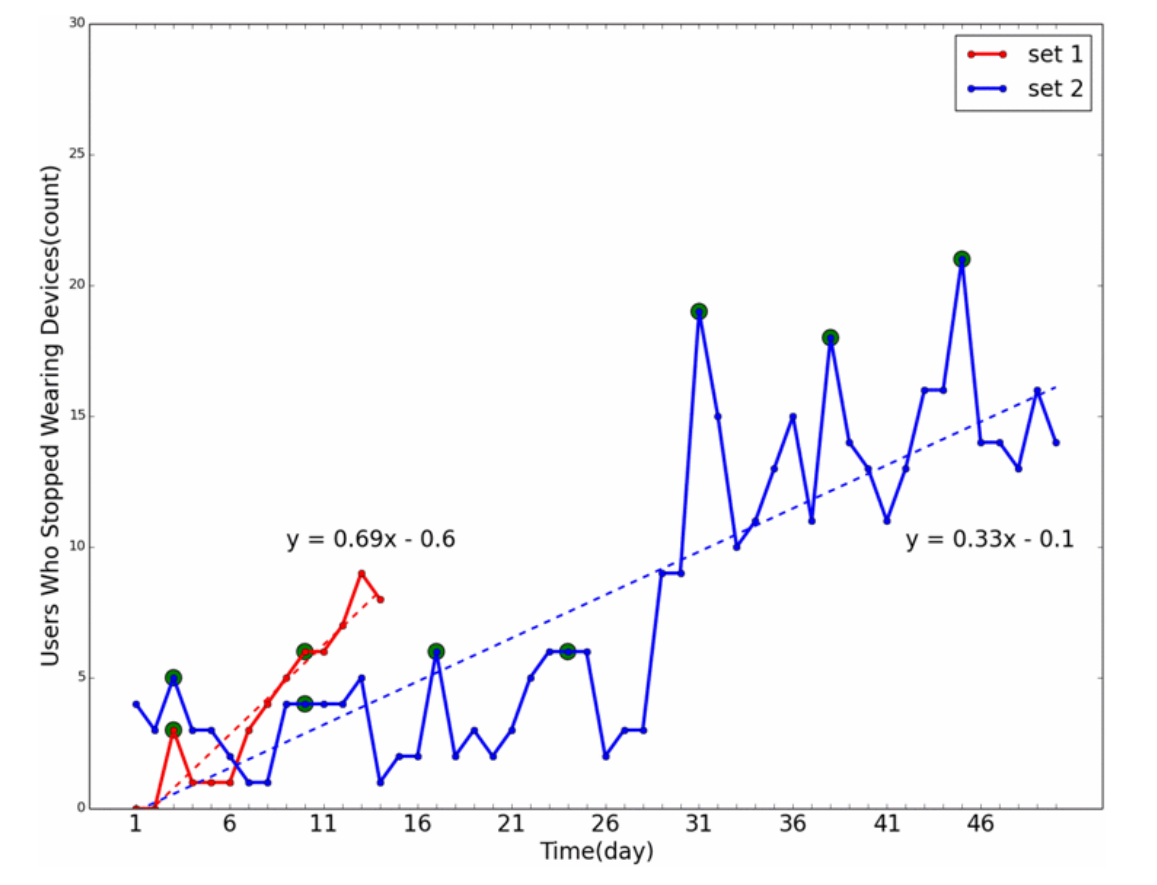
\includegraphics[scale=0.50]{figures/trackerAbandonment.png}
    \caption{Activity tracker abandonment rate \cite{Lee2017}}
    \label{acttrack}
\end{figure}

To try to deal with the problem of an inactive lifestyle and high abandonment rate of activity trackers and application, this project will develop a high-fidelity prototype with a focus on social cooperative fitness. The functionality from the prototype will log training data for friends, families or work place colleagues that have similar fitness goals in mind. The goal of the application is to encourage exercise and keep each member accountable of each other to promote physical health by achieving short-term and long-term goals.

\textbf{The hypothesis is that the social logging functionality would improve the accountability and motivation for using activity trackers and applications by letting users stay accountable of each other with small groups where they can log their workouts and having both short-term and long-term goals.}

The scientific approach will be design science which provides methods where relevant solutions will be designed for real people and environments with the goal of contributing to the existing knowledge base. Working with the user group, potential users have been interviewed and presented with different design choices and contributed with their information needs and preferences. 


\section{Research Questions}
\begin{enumerate}
    \item Can social fitness functionality increase the use and motivation for working out for the users? 
    \item Does sharing the data in small groups encourage more activity among the members?
    \item Can the application features assist users in staying accountable for working out and logging their progress?
\end{enumerate}
\subsection{Goals}
The goals of the research are:
\begin{enumerate}
\item Identify what social group features works for fitness applications
\item Present feature recommendations which can be used by established fitness applications
\item Develop a prototype for testing the features
\item Do development iterations, implement feedback
 and present potential improvements of the prototype functionality 
\end{enumerate}
The goals of the features are to get users to staying accountable to working out and logging their workouts and progress while cooperating with friends and families to meet their personal and group goals.
 
\newpage
 
\section{Outline of research project}
The following is the outline of the research project:

\textbf{Chapter 2: Sedentary lifestyle and benefits of exercise} Shows the dangers of sedentary lifestyle, explains exercise and strength training, looks at how people are motivated and benefits of exercise.

\textbf{Chapter 3: Literature review} Summarises the literature and related work for this project, relevant literature in human computer-interaction and computer supported cooperative work. References studies done with work colleagues, friends, how information is shared and the social incentives for fitness applications. Overview over fitness tracking and devices and the benefits of using them.

\textbf{Chapter 4: Methodologies} Explains the methodologies that are used in this project and the contributions

\textbf{Chapter 5: Requirements} Shows ethical considerations, the target group, participants of the project and the requirements that was gathered from the users

\textbf{Chapter 6: Prototype development} Shows the design iteration, the scientific process and summaries of each iteration from the user feedback

\textbf{Chapter 7: Features of application} Shows the high-fidelity prototype and the functionalities

\textbf{Chapter 8: Evaluation} Summarises the results from all the evaluations from this project

\textbf{Chapter 9: Discussion} Answers the research questions and the use of the different methodologies and the development process

\textbf{Chapter 10: Conclusion and future work} Concludes the project and recommendations for future work




